% Generated by Sphinx.
\def\sphinxdocclass{report}
\documentclass[letterpaper,10pt,english]{sphinxmanual}
\usepackage[utf8]{inputenc}
\DeclareUnicodeCharacter{00A0}{\nobreakspace}
\usepackage{cmap}
\usepackage[T1]{fontenc}
\usepackage{babel}
\usepackage{times}
\usepackage[Bjarne]{fncychap}
\usepackage{longtable}
\usepackage{sphinx}
\usepackage{multirow}


\title{Onitu Documentation}
\date{March 16, 2014}
\release{0.1-prev}
\author{Yannick PÉROUX, Alexandre Baron, Antoine Rozo, Wannes Rombouts, Louis Roche, Maxime Constantinian, Morgan Faget, Mathis Dupuy}
\newcommand{\sphinxlogo}{}
\renewcommand{\releasename}{Release}
\makeindex

\makeatletter
\def\PYG@reset{\let\PYG@it=\relax \let\PYG@bf=\relax%
    \let\PYG@ul=\relax \let\PYG@tc=\relax%
    \let\PYG@bc=\relax \let\PYG@ff=\relax}
\def\PYG@tok#1{\csname PYG@tok@#1\endcsname}
\def\PYG@toks#1+{\ifx\relax#1\empty\else%
    \PYG@tok{#1}\expandafter\PYG@toks\fi}
\def\PYG@do#1{\PYG@bc{\PYG@tc{\PYG@ul{%
    \PYG@it{\PYG@bf{\PYG@ff{#1}}}}}}}
\def\PYG#1#2{\PYG@reset\PYG@toks#1+\relax+\PYG@do{#2}}

\expandafter\def\csname PYG@tok@gd\endcsname{\def\PYG@tc##1{\textcolor[rgb]{0.63,0.00,0.00}{##1}}}
\expandafter\def\csname PYG@tok@gu\endcsname{\let\PYG@bf=\textbf\def\PYG@tc##1{\textcolor[rgb]{0.50,0.00,0.50}{##1}}}
\expandafter\def\csname PYG@tok@gt\endcsname{\def\PYG@tc##1{\textcolor[rgb]{0.00,0.27,0.87}{##1}}}
\expandafter\def\csname PYG@tok@gs\endcsname{\let\PYG@bf=\textbf}
\expandafter\def\csname PYG@tok@gr\endcsname{\def\PYG@tc##1{\textcolor[rgb]{1.00,0.00,0.00}{##1}}}
\expandafter\def\csname PYG@tok@cm\endcsname{\let\PYG@it=\textit\def\PYG@tc##1{\textcolor[rgb]{0.25,0.50,0.56}{##1}}}
\expandafter\def\csname PYG@tok@vg\endcsname{\def\PYG@tc##1{\textcolor[rgb]{0.73,0.38,0.84}{##1}}}
\expandafter\def\csname PYG@tok@m\endcsname{\def\PYG@tc##1{\textcolor[rgb]{0.13,0.50,0.31}{##1}}}
\expandafter\def\csname PYG@tok@mh\endcsname{\def\PYG@tc##1{\textcolor[rgb]{0.13,0.50,0.31}{##1}}}
\expandafter\def\csname PYG@tok@cs\endcsname{\def\PYG@tc##1{\textcolor[rgb]{0.25,0.50,0.56}{##1}}\def\PYG@bc##1{\setlength{\fboxsep}{0pt}\colorbox[rgb]{1.00,0.94,0.94}{\strut ##1}}}
\expandafter\def\csname PYG@tok@ge\endcsname{\let\PYG@it=\textit}
\expandafter\def\csname PYG@tok@vc\endcsname{\def\PYG@tc##1{\textcolor[rgb]{0.73,0.38,0.84}{##1}}}
\expandafter\def\csname PYG@tok@il\endcsname{\def\PYG@tc##1{\textcolor[rgb]{0.13,0.50,0.31}{##1}}}
\expandafter\def\csname PYG@tok@go\endcsname{\def\PYG@tc##1{\textcolor[rgb]{0.20,0.20,0.20}{##1}}}
\expandafter\def\csname PYG@tok@cp\endcsname{\def\PYG@tc##1{\textcolor[rgb]{0.00,0.44,0.13}{##1}}}
\expandafter\def\csname PYG@tok@gi\endcsname{\def\PYG@tc##1{\textcolor[rgb]{0.00,0.63,0.00}{##1}}}
\expandafter\def\csname PYG@tok@gh\endcsname{\let\PYG@bf=\textbf\def\PYG@tc##1{\textcolor[rgb]{0.00,0.00,0.50}{##1}}}
\expandafter\def\csname PYG@tok@ni\endcsname{\let\PYG@bf=\textbf\def\PYG@tc##1{\textcolor[rgb]{0.84,0.33,0.22}{##1}}}
\expandafter\def\csname PYG@tok@nl\endcsname{\let\PYG@bf=\textbf\def\PYG@tc##1{\textcolor[rgb]{0.00,0.13,0.44}{##1}}}
\expandafter\def\csname PYG@tok@nn\endcsname{\let\PYG@bf=\textbf\def\PYG@tc##1{\textcolor[rgb]{0.05,0.52,0.71}{##1}}}
\expandafter\def\csname PYG@tok@no\endcsname{\def\PYG@tc##1{\textcolor[rgb]{0.38,0.68,0.84}{##1}}}
\expandafter\def\csname PYG@tok@na\endcsname{\def\PYG@tc##1{\textcolor[rgb]{0.25,0.44,0.63}{##1}}}
\expandafter\def\csname PYG@tok@nb\endcsname{\def\PYG@tc##1{\textcolor[rgb]{0.00,0.44,0.13}{##1}}}
\expandafter\def\csname PYG@tok@nc\endcsname{\let\PYG@bf=\textbf\def\PYG@tc##1{\textcolor[rgb]{0.05,0.52,0.71}{##1}}}
\expandafter\def\csname PYG@tok@nd\endcsname{\let\PYG@bf=\textbf\def\PYG@tc##1{\textcolor[rgb]{0.33,0.33,0.33}{##1}}}
\expandafter\def\csname PYG@tok@ne\endcsname{\def\PYG@tc##1{\textcolor[rgb]{0.00,0.44,0.13}{##1}}}
\expandafter\def\csname PYG@tok@nf\endcsname{\def\PYG@tc##1{\textcolor[rgb]{0.02,0.16,0.49}{##1}}}
\expandafter\def\csname PYG@tok@si\endcsname{\let\PYG@it=\textit\def\PYG@tc##1{\textcolor[rgb]{0.44,0.63,0.82}{##1}}}
\expandafter\def\csname PYG@tok@s2\endcsname{\def\PYG@tc##1{\textcolor[rgb]{0.25,0.44,0.63}{##1}}}
\expandafter\def\csname PYG@tok@vi\endcsname{\def\PYG@tc##1{\textcolor[rgb]{0.73,0.38,0.84}{##1}}}
\expandafter\def\csname PYG@tok@nt\endcsname{\let\PYG@bf=\textbf\def\PYG@tc##1{\textcolor[rgb]{0.02,0.16,0.45}{##1}}}
\expandafter\def\csname PYG@tok@nv\endcsname{\def\PYG@tc##1{\textcolor[rgb]{0.73,0.38,0.84}{##1}}}
\expandafter\def\csname PYG@tok@s1\endcsname{\def\PYG@tc##1{\textcolor[rgb]{0.25,0.44,0.63}{##1}}}
\expandafter\def\csname PYG@tok@gp\endcsname{\let\PYG@bf=\textbf\def\PYG@tc##1{\textcolor[rgb]{0.78,0.36,0.04}{##1}}}
\expandafter\def\csname PYG@tok@sh\endcsname{\def\PYG@tc##1{\textcolor[rgb]{0.25,0.44,0.63}{##1}}}
\expandafter\def\csname PYG@tok@ow\endcsname{\let\PYG@bf=\textbf\def\PYG@tc##1{\textcolor[rgb]{0.00,0.44,0.13}{##1}}}
\expandafter\def\csname PYG@tok@sx\endcsname{\def\PYG@tc##1{\textcolor[rgb]{0.78,0.36,0.04}{##1}}}
\expandafter\def\csname PYG@tok@bp\endcsname{\def\PYG@tc##1{\textcolor[rgb]{0.00,0.44,0.13}{##1}}}
\expandafter\def\csname PYG@tok@c1\endcsname{\let\PYG@it=\textit\def\PYG@tc##1{\textcolor[rgb]{0.25,0.50,0.56}{##1}}}
\expandafter\def\csname PYG@tok@kc\endcsname{\let\PYG@bf=\textbf\def\PYG@tc##1{\textcolor[rgb]{0.00,0.44,0.13}{##1}}}
\expandafter\def\csname PYG@tok@c\endcsname{\let\PYG@it=\textit\def\PYG@tc##1{\textcolor[rgb]{0.25,0.50,0.56}{##1}}}
\expandafter\def\csname PYG@tok@mf\endcsname{\def\PYG@tc##1{\textcolor[rgb]{0.13,0.50,0.31}{##1}}}
\expandafter\def\csname PYG@tok@err\endcsname{\def\PYG@bc##1{\setlength{\fboxsep}{0pt}\fcolorbox[rgb]{1.00,0.00,0.00}{1,1,1}{\strut ##1}}}
\expandafter\def\csname PYG@tok@kd\endcsname{\let\PYG@bf=\textbf\def\PYG@tc##1{\textcolor[rgb]{0.00,0.44,0.13}{##1}}}
\expandafter\def\csname PYG@tok@ss\endcsname{\def\PYG@tc##1{\textcolor[rgb]{0.32,0.47,0.09}{##1}}}
\expandafter\def\csname PYG@tok@sr\endcsname{\def\PYG@tc##1{\textcolor[rgb]{0.14,0.33,0.53}{##1}}}
\expandafter\def\csname PYG@tok@mo\endcsname{\def\PYG@tc##1{\textcolor[rgb]{0.13,0.50,0.31}{##1}}}
\expandafter\def\csname PYG@tok@mi\endcsname{\def\PYG@tc##1{\textcolor[rgb]{0.13,0.50,0.31}{##1}}}
\expandafter\def\csname PYG@tok@kn\endcsname{\let\PYG@bf=\textbf\def\PYG@tc##1{\textcolor[rgb]{0.00,0.44,0.13}{##1}}}
\expandafter\def\csname PYG@tok@o\endcsname{\def\PYG@tc##1{\textcolor[rgb]{0.40,0.40,0.40}{##1}}}
\expandafter\def\csname PYG@tok@kr\endcsname{\let\PYG@bf=\textbf\def\PYG@tc##1{\textcolor[rgb]{0.00,0.44,0.13}{##1}}}
\expandafter\def\csname PYG@tok@s\endcsname{\def\PYG@tc##1{\textcolor[rgb]{0.25,0.44,0.63}{##1}}}
\expandafter\def\csname PYG@tok@kp\endcsname{\def\PYG@tc##1{\textcolor[rgb]{0.00,0.44,0.13}{##1}}}
\expandafter\def\csname PYG@tok@w\endcsname{\def\PYG@tc##1{\textcolor[rgb]{0.73,0.73,0.73}{##1}}}
\expandafter\def\csname PYG@tok@kt\endcsname{\def\PYG@tc##1{\textcolor[rgb]{0.56,0.13,0.00}{##1}}}
\expandafter\def\csname PYG@tok@sc\endcsname{\def\PYG@tc##1{\textcolor[rgb]{0.25,0.44,0.63}{##1}}}
\expandafter\def\csname PYG@tok@sb\endcsname{\def\PYG@tc##1{\textcolor[rgb]{0.25,0.44,0.63}{##1}}}
\expandafter\def\csname PYG@tok@k\endcsname{\let\PYG@bf=\textbf\def\PYG@tc##1{\textcolor[rgb]{0.00,0.44,0.13}{##1}}}
\expandafter\def\csname PYG@tok@se\endcsname{\let\PYG@bf=\textbf\def\PYG@tc##1{\textcolor[rgb]{0.25,0.44,0.63}{##1}}}
\expandafter\def\csname PYG@tok@sd\endcsname{\let\PYG@it=\textit\def\PYG@tc##1{\textcolor[rgb]{0.25,0.44,0.63}{##1}}}

\def\PYGZbs{\char`\\}
\def\PYGZus{\char`\_}
\def\PYGZob{\char`\{}
\def\PYGZcb{\char`\}}
\def\PYGZca{\char`\^}
\def\PYGZam{\char`\&}
\def\PYGZlt{\char`\<}
\def\PYGZgt{\char`\>}
\def\PYGZsh{\char`\#}
\def\PYGZpc{\char`\%}
\def\PYGZdl{\char`\$}
\def\PYGZhy{\char`\-}
\def\PYGZsq{\char`\'}
\def\PYGZdq{\char`\"}
\def\PYGZti{\char`\~}
% for compatibility with earlier versions
\def\PYGZat{@}
\def\PYGZlb{[}
\def\PYGZrb{]}
\makeatother

\begin{document}

\maketitle
\tableofcontents
\phantomsection\label{index::doc}


Onitu is a tool that can synchronize files between various places. This documentation contains everything you need to know in order to start hacking Onitu.

\begin{notice}{note}{Note:}
This is a technical documentation. If you want to learn how to use Onitu, you should take a look at our \href{http://github.com/onitu/onitu}{User Documentation}.
\end{notice}


\chapter{Content table}
\label{index:onitu-version-technical-documentation}\label{index:content-table}\label{index:user-documentation}

\section{Getting started}
\label{intro:getting-started}\label{intro::doc}

\subsection{Onitu at a glance}
\label{intro:onitu-at-a-glance}
Onitu must deal with a lot of events coming from different places. Therefore, Onitu is build around an asynchronous model. Each part runs in a separate process, and communicate with the others via ZeroMQ messages and Redis.

In order to synchronize files between external services, Onitu uses a system of drivers. You can find more information about this system in {\hyperref[drivers::doc]{\emph{Creating a new driver}}}. Each driver sends events and receives orders from the {\hyperref[components:onitu.referee.Referee]{\code{Referee}}}, which chooses where the files should be synchronised according to the configuration rules.


\subsection{Glossary}
\label{intro:glossary}\begin{description}
\item[{\index{Driver|textbf}Driver}] \leavevmode\phantomsection\label{intro:term-driver}
A program making the junction between Onitu and a remote service (SSH, Dropbox, a hard drive…). \emph{cf} {\hyperref[drivers::doc]{\emph{Creating a new driver}}}

\item[{\index{Entry|textbf}Entry}] \leavevmode\phantomsection\label{intro:term-entry}
A driver configured by the user. For example, it can be the Dropbox driver configured to run with a specific account. You can view an entry as an instance of a driver.

\item[{\index{Rule|textbf}Rule}] \leavevmode\phantomsection\label{intro:term-rule}
Maps a set of matching files to a set of entries. Used in the configuration to split up the files.

\item[{\index{Setup|textbf}Setup}] \leavevmode\phantomsection\label{intro:term-setup}
A JSON configuration file, which describes the entries and the rules.

\item[{\index{Referee|textbf}Referee}] \leavevmode\phantomsection\label{intro:term-referee}
Receive events from the drivers and allocate the files among the entries regarding the configuration rules. \emph{cf} {\hyperref[components:onitu.referee.Referee]{\code{Referee}}}

\item[{\index{Plug|textbf}Plug}] \leavevmode\phantomsection\label{intro:term-plug}
A helper class which implements all the boilerplate needed by a driver to communicate with Onitu. \emph{cf} {\hyperref[drivers:onitu.api.Plug]{\code{Plug}}}

\item[{\index{Handler|textbf}Handler}] \leavevmode\phantomsection\label{intro:term-handler}
A function defined by a driver, which responds to a specific task. This function will be called by the {\hyperref[drivers:onitu.api.Plug]{\code{Plug}}} when needed. \emph{cf} {\hyperref[drivers:handlers]{\emph{Handlers}}}

\end{description}


\subsection{Global architecture}
\label{intro:global-architecture}
You can here find an illustration of the global architecture of Onitu: {\hyperref[intro:schematic]{\emph{Figure 1.1}}}.
\begin{figure}[htbp]
\centering
\capstart

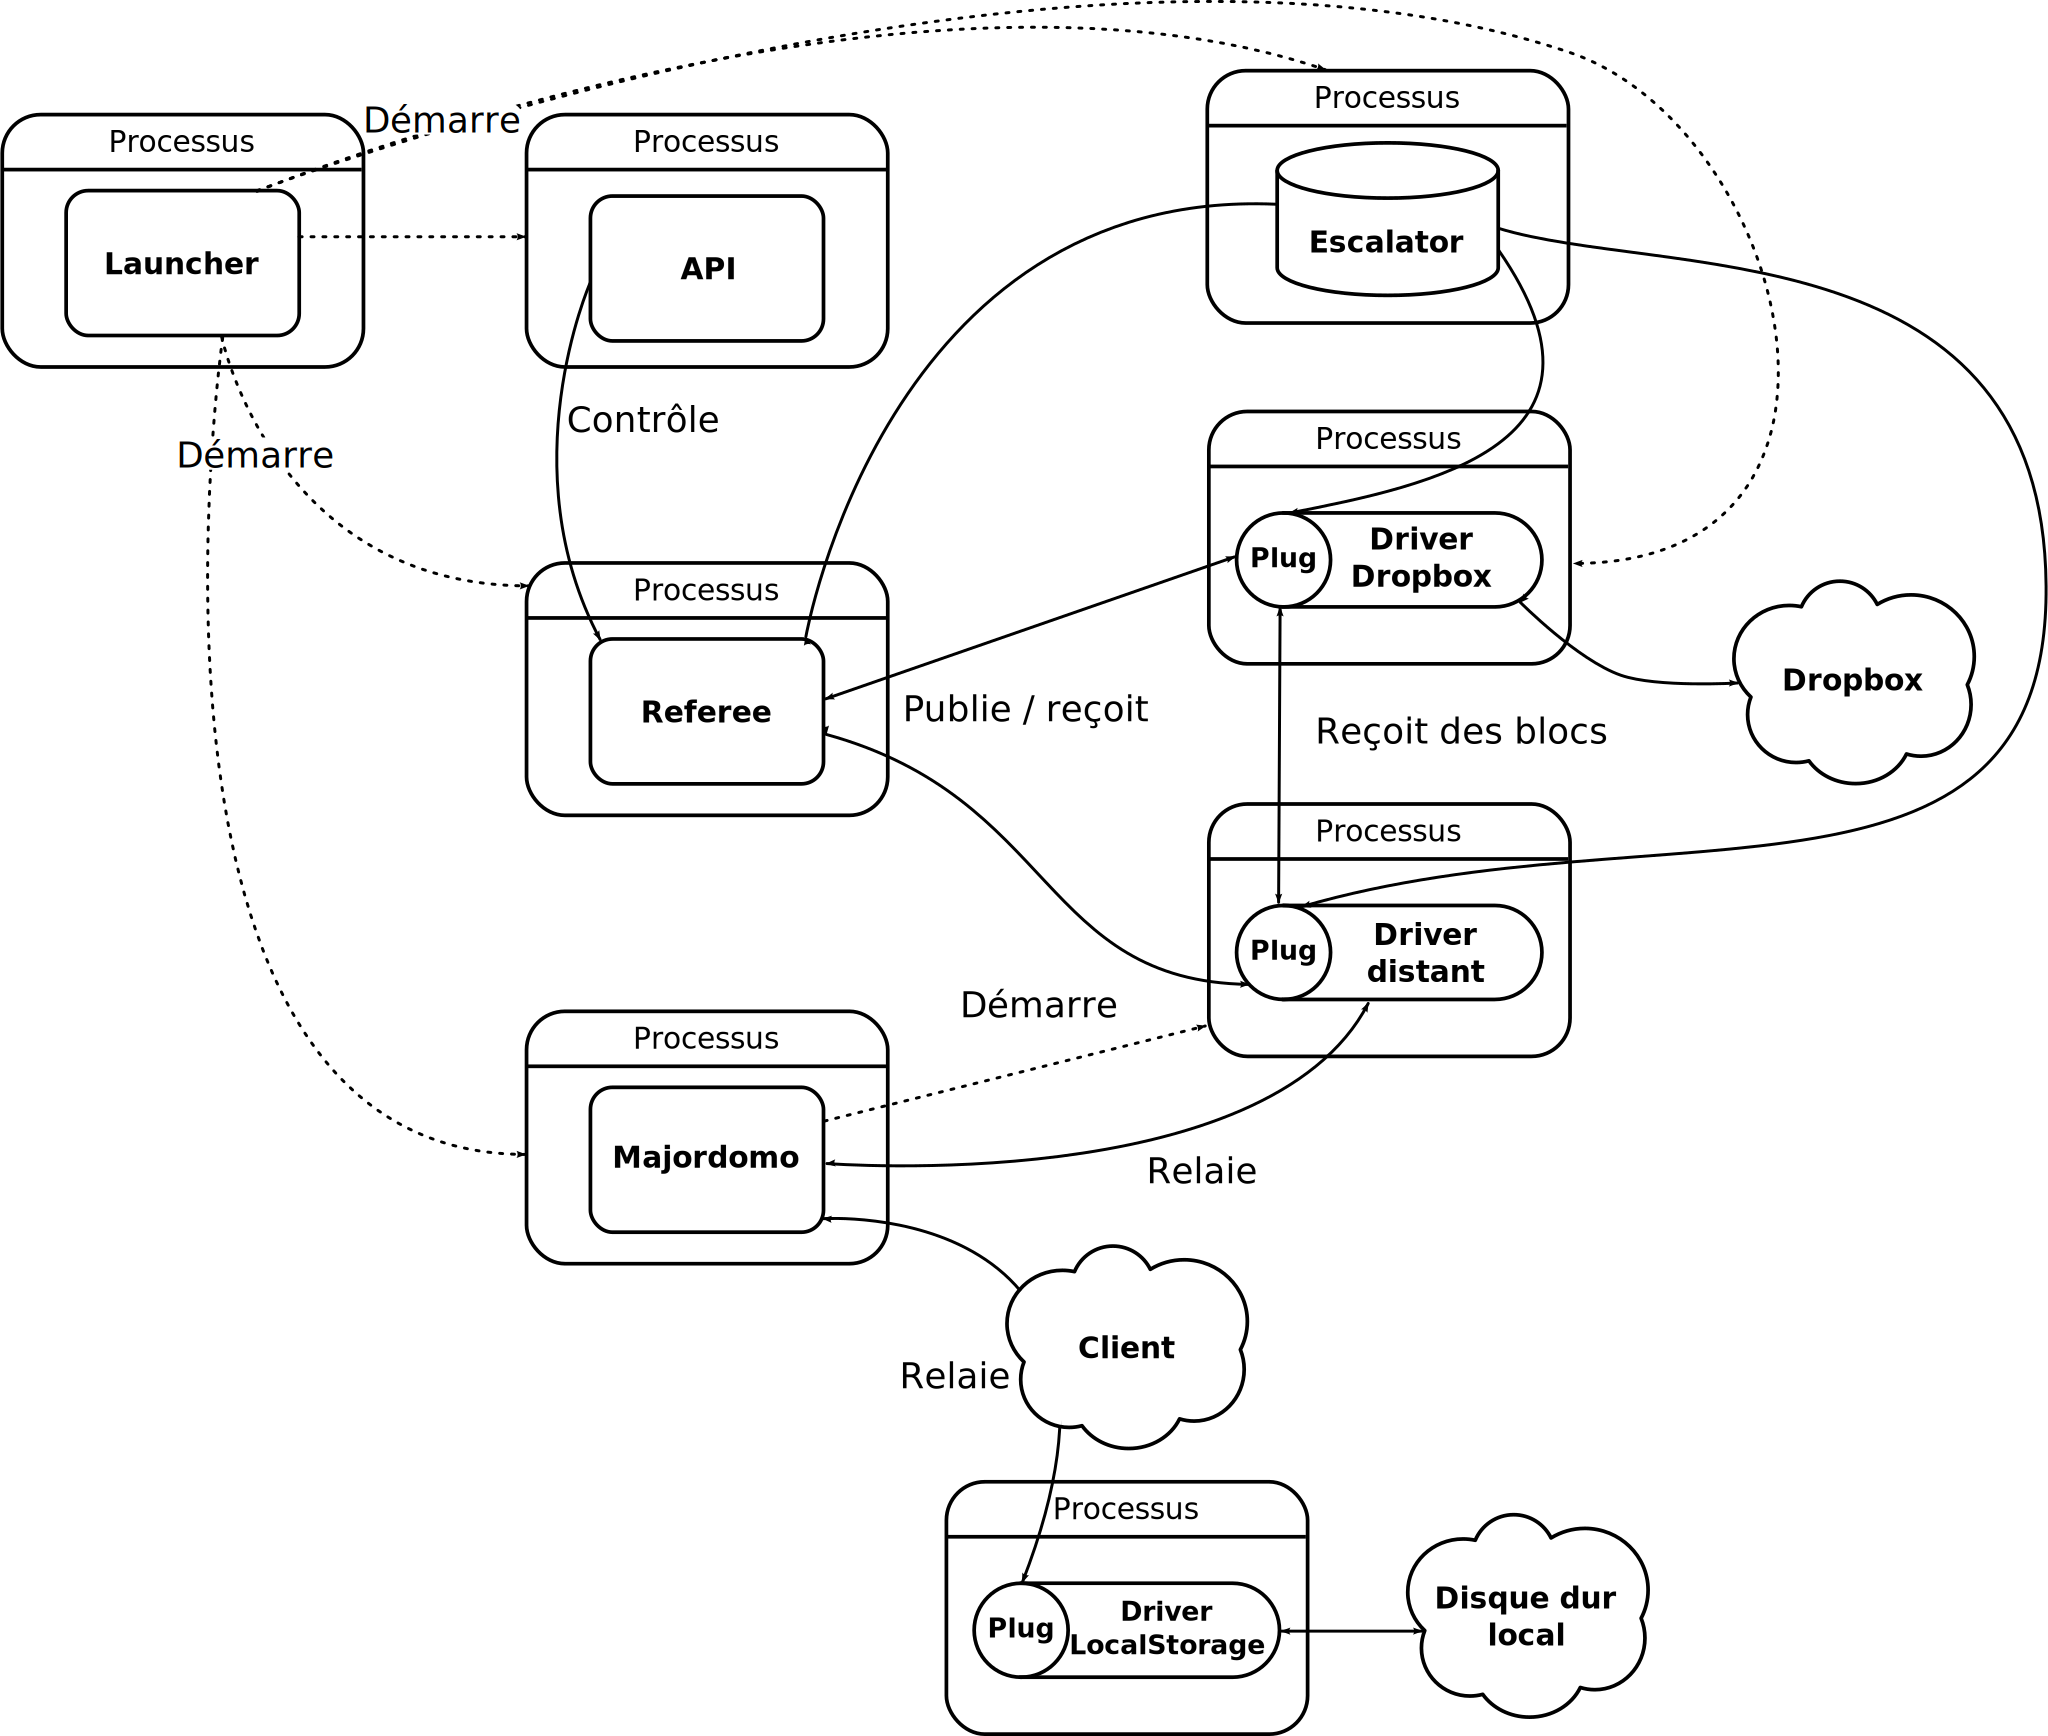
\includegraphics{global_archi.png}
\caption{A schematic illustrating the global architecture of Onitu with two drivers.}\label{intro:schematic}\end{figure}


\subsection{Dependencies}
\label{intro:dependencies}
The core of Onitu uses several libraries (other dependencies exists but are specific to some drivers):
\begin{description}
\item[{\href{http://circus.readthedocs.org}{Circus}}] \leavevmode
Used to start, manage and monitor the different processes

\item[{\href{http://github.com/zeromq/pyzmq}{PyZMQ}}] \leavevmode
A binding of the ZeroMQ library for the Python language

\item[{\href{http://github.com/andymccurdy/redis-py}{redis-py}}] \leavevmode
A library to communicate with Redis in Python

\item[{\href{http://pythonhosted.org/Logbook/}{Logbook}}] \leavevmode
A powerful logging library that allows Onitu to log on a ZeroMQ channel, aggregating all the logs in the same place

\end{description}


\subsection{Technical choices}
\label{intro:logbook}\label{intro:technical-choices}
We made some difficult technical choices in order to build Onitu in the most maintainable and efficient way. Those choices can be questionable, but here are our motivations :


\subsubsection{Python}
\label{intro:python}
Python is a general-purpose and flexible language. This was our first choice because all of us were already using and loving it. It allows us to distribute Onitu easily, without having to compile the sources or distribute binaries. Python is available on a lot of different systems, has a lot of built-in functionalities and is easy to understand and read.

You might have some concerns regarding the speed, but Onitu is an I/O bound application, so most of the time it is not executing Python code but downloading/uploading files or exchanging information over sockets. The same program with a low-level language like C would introduce a lot of complexity and probably only a very small performance amelioration.


\subsubsection{ZeroMQ}
\label{intro:zeromq}
As Onitu is an application with a lot of different processes and threads, we need a way to communicate between them. ZeroMQ is a layer on top of IP and Unix sockets, and provides messaging patterns. Onitu uses several of them, like ROUTER/DEALER, PUBLISH/SUBSCRIBE and REQUEST/REPLY.

ZeroMQ is really fast, available on a lot of platforms and has Python bindings. It is much more flexible and lightweight than other message brockers, such as RabbitMQ or ActiveMQ.


\subsubsection{Redis}
\label{intro:redis}
Onitu needs to store information in a persistent database. This database should be cross-platform, schema-less and easy to install and maintain. For that purpose, Redis has been chosen. But Redis is not available in the same version on all platforms, and is not really persistent. Also, the entire database is in-memory, limiting its size. Therefore, another solution will soon be chosen to replace it as it is not the perfect solution.


\section{Creating a new driver}
\label{drivers:creating-a-new-driver}\label{drivers::doc}
A driver is a Python program that allows Onitu to synchronize files with a remote service, such as Dropbox, Google Drive, SSH, FTP or a local hard drive.


\subsection{Basics}
\label{drivers:basics}
The drivers communicate with Onitu via the {\hyperref[drivers:onitu.api.Plug]{\code{Plug}}} class, which handles the operations common to all drivers. Each driver implements its specific tasks with the system of {\hyperref[drivers:handlers]{handlers}}. Those handlers will be called by the {\hyperref[drivers:onitu.api.Plug]{\code{Plug}}} at certain occasions.

In Onitu the file transfers are made by chunks. When a new transfer begin, the {\hyperref[drivers:onitu.api.Plug]{\code{Plug}}} asks the others drivers for new chunks, and then call the \emph{upload\_chunk} handler.

Each driver should expose a function called \emph{start}, which takes a name as first parameter, and returns nothing. The name is chosen by the user when he configures the driver.
This function will be called by Onitu during the initialization of the driver, and should not return until the end of life of the driver (\emph{cf} {\hyperref[drivers:onitu.api.Plug.listen]{\code{Plug.listen()}}}).

When a driver detects an update in a file, it should update the {\hyperref[drivers:onitu.api.metadata.Metadata]{\code{Metadata}}} of the file, specify a {\hyperref[drivers:onitu.api.metadata.Metadata.revision]{\code{Metadata.revision}}}, and call :meth.{}`.Plug.update\_file{}`.

\begin{notice}{note}{Note:}
During their startup, the drivers should look for new files or updates on their remote file system. They should also listen to changes during their lifetime. The mechanism used to do that is specific to each driver, and can't be abstracted by the {\hyperref[drivers:onitu.api.Plug]{\code{Plug}}}.
\end{notice}

Onitu provide a set of {\hyperref[contribute:tests]{\emph{functional tests}}} that you can use to see if your driver respond to every exigence.


\subsection{Handlers}
\label{drivers:id1}\label{drivers:handlers}
A handler is a function that will be called by the Plug on different occasions, such as getting a chunk from a file or starting a transfer. The drivers can define any handler they need. For example, some driver don't need to do anything for initiating a transfer, so they might not want to implement the \emph{end\_upload} handler.
In order to register a handler, the {\hyperref[drivers:onitu.api.Plug.handler]{\code{Plug.handler()}}} decorator is used.

\begin{notice}{warning}{Warning:}
All the handlers \textbf{must be thread-safe}. The plug uses several threads to handle concurrent requests, and each handler can be called from any of those threads. The {\hyperref[drivers:onitu.api.Plug]{\code{Plug}}} itself is fully thread-safe.
\end{notice}

At this stage, the list of the handlers that can be defined is the following :
\index{get\_chunk() (built-in function)}

\begin{fulllineitems}
\phantomsection\label{drivers:get_chunk}\pysiglinewithargsret{\bfcode{get\_chunk}}{\emph{filename}, \emph{offset}, \emph{size}}{}
Return a chunk of a given size, starting at the given offset, from a file.
\begin{quote}\begin{description}
\item[{Parameters}] \leavevmode\begin{itemize}
\item {} 
\textbf{filename} (\emph{string}) -- The absolute path to the file

\item {} 
\textbf{offset} (\emph{int}) -- The offset from which the content should be retrieved

\item {} 
\textbf{size} (\emph{int}) -- The maximum size of the chunk that should be returned

\end{itemize}

\item[{Return type}] \leavevmode
string

\end{description}\end{quote}

\end{fulllineitems}

\index{upload\_chunk() (built-in function)}

\begin{fulllineitems}
\phantomsection\label{drivers:upload_chunk}\pysiglinewithargsret{\bfcode{upload\_chunk}}{\emph{filename}, \emph{offset}, \emph{chunk}}{}
Write a chunk in a file at a given offset.
\begin{quote}\begin{description}
\item[{Parameters}] \leavevmode\begin{itemize}
\item {} 
\textbf{filename} (\emph{string}) -- The absolute path to the file

\item {} 
\textbf{offset} (\emph{int}) -- The offset from which the content should be written

\item {} 
\textbf{chunk} (\emph{string}) -- The content that should be written

\end{itemize}

\end{description}\end{quote}

\end{fulllineitems}

\index{start\_upload() (built-in function)}

\begin{fulllineitems}
\phantomsection\label{drivers:start_upload}\pysiglinewithargsret{\bfcode{start\_upload}}{\emph{metadata}}{}
Initialize a new upload. This handler is called when a new transfer is started.
\begin{quote}\begin{description}
\item[{Parameters}] \leavevmode
\textbf{metadata} ({\hyperref[drivers:onitu.api.metadata.Metadata]{\code{Metadata}}}) -- The metadata of the file transferred

\end{description}\end{quote}

\end{fulllineitems}

\index{restart\_upload() (built-in function)}

\begin{fulllineitems}
\phantomsection\label{drivers:restart_upload}\pysiglinewithargsret{\bfcode{restart\_upload}}{\emph{metadata}, \emph{offset}}{}
Restart a failed upload. This handler will be called during the startup if a transfer has been stopped.
\begin{quote}\begin{description}
\item[{Parameters}] \leavevmode\begin{itemize}
\item {} 
\textbf{metadata} ({\hyperref[drivers:onitu.api.metadata.Metadata]{\code{Metadata}}}) -- The metadata of the file transferred

\item {} 
\textbf{offset} (\emph{int}) -- The offset of the last chunk uploaded

\end{itemize}

\end{description}\end{quote}

\end{fulllineitems}

\index{end\_upload() (built-in function)}

\begin{fulllineitems}
\phantomsection\label{drivers:end_upload}\pysiglinewithargsret{\bfcode{end\_upload}}{\emph{metadata}}{}
Called when a transfer is over.
\begin{quote}\begin{description}
\item[{Parameters}] \leavevmode
\textbf{metadata} ({\hyperref[drivers:onitu.api.metadata.Metadata]{\code{Metadata}}}) -- The metadata of the file transferred

\end{description}\end{quote}

\end{fulllineitems}

\index{abort\_upload() (built-in function)}

\begin{fulllineitems}
\phantomsection\label{drivers:abort_upload}\pysiglinewithargsret{\bfcode{abort\_upload}}{\emph{metadata}}{}
Called when a transfer is aborted. For example, this could happen if a newer version of the file should be uploaded during the transfer.
\begin{quote}\begin{description}
\item[{Parameters}] \leavevmode
\textbf{metadata} ({\hyperref[drivers:onitu.api.metadata.Metadata]{\code{Metadata}}}) -- The metadata of the file transferred

\end{description}\end{quote}

\end{fulllineitems}



\subsection{The Plug}
\label{drivers:the-plug}\index{Plug (class in onitu.api)}

\begin{fulllineitems}
\phantomsection\label{drivers:onitu.api.Plug}\pysigline{\strong{class }\code{onitu.api.}\bfcode{Plug}}
The Plug is the preferred way for a driver to communicate
with other drivers, the {\hyperref[components:onitu.referee.Referee]{\code{Referee}}}, or
the database.

Each driver must instantiate a new Plug, and define handlers
(see {\hyperref[drivers:onitu.api.Plug.handler]{\code{handler()}}}).

{\hyperref[drivers:onitu.api.Plug.initialize]{\code{initialize()}}} should be called at the beginning of the
\emph{start} function, and
When it is ready to receive requests from other drivers,
it should call {\hyperref[components:onitu.referee.Referee.listen]{\code{listen()}}}. This function blocks until
the driver is shut down.
\index{get\_metadata() (onitu.api.Plug method)}

\begin{fulllineitems}
\phantomsection\label{drivers:onitu.api.Plug.get_metadata}\pysiglinewithargsret{\bfcode{get\_metadata}}{\emph{filename}}{}~\begin{quote}\begin{description}
\item[{Parameters}] \leavevmode
\textbf{filename} -- The name of the file, with the absolute path
from the driver's root

\item[{Return type}] \leavevmode
{\hyperref[drivers:onitu.api.metadata.Metadata]{\code{Metadata}}}

\end{description}\end{quote}

If the file does not exists in Onitu, it will be created when
{\hyperref[drivers:onitu.api.metadata.Metadata.write]{\code{Metadata.write()}}} will be called.

\end{fulllineitems}

\index{handler() (onitu.api.Plug method)}

\begin{fulllineitems}
\phantomsection\label{drivers:onitu.api.Plug.handler}\pysiglinewithargsret{\bfcode{handler}}{\emph{task=None}}{}
Decorator used register a handler for a particular task.
\begin{quote}\begin{description}
\item[{Parameters}] \leavevmode
\textbf{task} (\emph{string}) -- Optional. The name of the handler. If not
specified, the name of the function will be used.

\end{description}\end{quote}

Example:

\begin{Verbatim}[commandchars=\\\{\}]
\PYG{n+nd}{@plug.handler}\PYG{p}{(}\PYG{p}{)}
\PYG{k}{def} \PYG{n+nf}{get\PYGZus{}chunk}\PYG{p}{(}\PYG{n}{filename}\PYG{p}{,} \PYG{n}{offset}\PYG{p}{,} \PYG{n}{size}\PYG{p}{)}\PYG{p}{:}
    \PYG{k}{with} \PYG{n+nb}{open}\PYG{p}{(}\PYG{n}{filename}\PYG{p}{,} \PYG{l+s}{\PYGZsq{}}\PYG{l+s}{rb}\PYG{l+s}{\PYGZsq{}}\PYG{p}{)} \PYG{k}{as} \PYG{n}{f}\PYG{p}{:}
        \PYG{n}{f}\PYG{o}{.}\PYG{n}{seek}\PYG{p}{(}\PYG{n}{offset}\PYG{p}{)}
        \PYG{k}{return} \PYG{n}{f}\PYG{o}{.}\PYG{n}{read}\PYG{p}{(}\PYG{n}{size}\PYG{p}{)}
\end{Verbatim}

\end{fulllineitems}

\index{initialize() (onitu.api.Plug method)}

\begin{fulllineitems}
\phantomsection\label{drivers:onitu.api.Plug.initialize}\pysiglinewithargsret{\bfcode{initialize}}{\emph{name}}{}
Initialize the different components of the Plug. The
drivers should call it in the beginning of the \emph{start}
function.
\begin{quote}\begin{description}
\item[{Parameters}] \leavevmode
\textbf{name} (\emph{string}) -- The name of the current entry, as given in
the \emph{start} function.

\end{description}\end{quote}

\end{fulllineitems}

\index{listen() (onitu.api.Plug method)}

\begin{fulllineitems}
\phantomsection\label{drivers:onitu.api.Plug.listen}\pysiglinewithargsret{\bfcode{listen}}{\emph{wait=True}}{}
Start listening to requests from other drivers or the
{\hyperref[components:onitu.referee.Referee]{\code{Referee}}}.
\begin{quote}\begin{description}
\item[{Parameters}] \leavevmode
\textbf{wait} (\emph{bool}) -- Optional. If true, blocks until the Plug is
killed. Default to True.

\end{description}\end{quote}

This method starts two threads :
\begin{itemize}
\item {} \index{Plug.Router (class in onitu.api.router)}

\begin{fulllineitems}
\phantomsection\label{drivers:onitu.api.router.Plug.Router}\pysiglinewithargsret{\strong{class }\bfcode{Router}}{\emph{plug}}{}
Receive and reply to requests from other drivers. This is the
component which calls the \emph{get\_chunk} handler.
It uses a single thread, which means that only one call to
\emph{get\_chunk} can be made at a time.

\end{fulllineitems}


\item {} \index{Dealer (class in onitu.api.dealer)}

\begin{fulllineitems}
\phantomsection\label{drivers:onitu.api.dealer.Dealer}\pysiglinewithargsret{\strong{class }\code{onitu.api.dealer.}\bfcode{Dealer}}{\emph{plug}}{}
Receive and reply to orders from the Referee.

All the requests are handled in a thread-pool.

\end{fulllineitems}


\end{itemize}

\end{fulllineitems}

\index{update\_file() (onitu.api.Plug method)}

\begin{fulllineitems}
\phantomsection\label{drivers:onitu.api.Plug.update_file}\pysiglinewithargsret{\code{Plug.}\bfcode{update\_file}}{\emph{metadata}}{}
This method should be called by the driver after each update
of a file or after the creation of a file.
It takes a {\hyperref[drivers:onitu.api.metadata.Metadata]{\code{Metadata}}} object in parameter that should have been
updated with the new value of the properties.

\end{fulllineitems}


\end{fulllineitems}



\subsection{Metadata}
\label{drivers:metadata}\index{Metadata (class in onitu.api.metadata)}

\begin{fulllineitems}
\phantomsection\label{drivers:onitu.api.metadata.Metadata}\pysiglinewithargsret{\strong{class }\code{onitu.api.metadata.}\bfcode{Metadata}}{\emph{plug=None}, \emph{filename=None}, \emph{size=0}}{}
The Metadata class represent the metadata of any file in Onitu.

This class should always be instantiated via the
{\hyperref[drivers:onitu.api.metadata.Metadata.get_by_id]{\code{get\_by\_id()}}} or {\hyperref[drivers:onitu.api.metadata.Metadata.get_by_filename]{\code{get\_by\_filename()}}}
class methods.
However, the drivers should never instantiate a new
{\hyperref[drivers:onitu.api.metadata.Metadata]{\code{Metadata}}} object themselves, but use the
{\hyperref[drivers:onitu.api.Plug.get_metadata]{\code{Plug.get\_metadata()}}} function.

The attributes available for each file are the following :
\begin{description}
\item[{\textbf{filename}}] \leavevmode
The absolute filename of the file

\item[{\textbf{size}}] \leavevmode
The size of the file, in octets

\item[{\textbf{revision}}] \leavevmode
This field is specific to each entry. It is a string
representing the current revision of the file for the
current entry.
The drivers should compare an upstream and a local version
of a file with this field. The format is dependant from the
driver (it can be whatever you want: a timestamp, a number,
a hash...).

\item[{\textbf{owners}}] \leavevmode
The entries which should have this file

\item[{\textbf{uptodate}}] \leavevmode
The entries with an up-to-date version of this file

\end{description}
\index{get\_by\_filename() (onitu.api.metadata.Metadata class method)}

\begin{fulllineitems}
\phantomsection\label{drivers:onitu.api.metadata.Metadata.get_by_filename}\pysiglinewithargsret{\strong{classmethod }\bfcode{get\_by\_filename}}{\emph{plug}, \emph{filename}}{}
Instantiate a new {\hyperref[drivers:onitu.api.metadata.Metadata]{\code{Metadata}}} object for the file
with the given name.

\end{fulllineitems}

\index{get\_by\_id() (onitu.api.metadata.Metadata class method)}

\begin{fulllineitems}
\phantomsection\label{drivers:onitu.api.metadata.Metadata.get_by_id}\pysiglinewithargsret{\strong{classmethod }\bfcode{get\_by\_id}}{\emph{plug}, \emph{fid}}{}
Instantiate a new {\hyperref[drivers:onitu.api.metadata.Metadata]{\code{Metadata}}} object for the file
with the given id.

\end{fulllineitems}

\index{revision (onitu.api.metadata.Metadata attribute)}

\begin{fulllineitems}
\phantomsection\label{drivers:onitu.api.metadata.Metadata.revision}\pysigline{\bfcode{revision}}
The revision of a file can be any string, and should be
used to compare the different versions of a file on driver.

Each driver can use its own system of revisions, as it is
stored for each entry.

\end{fulllineitems}

\index{write() (onitu.api.metadata.Metadata method)}

\begin{fulllineitems}
\phantomsection\label{drivers:onitu.api.metadata.Metadata.write}\pysiglinewithargsret{\bfcode{write}}{}{}
Write the metadata of the current file in the database.

\end{fulllineitems}

\index{write\_revision() (onitu.api.metadata.Metadata method)}

\begin{fulllineitems}
\phantomsection\label{drivers:onitu.api.metadata.Metadata.write_revision}\pysiglinewithargsret{\bfcode{write\_revision}}{}{}
Write the current revision in the database. Called
by {\hyperref[drivers:onitu.api.metadata.Metadata.write]{\code{write()}}}.

\end{fulllineitems}


\end{fulllineitems}



\subsection{Example}
\label{drivers:example}
Usually, the drivers are created as a set of functions in a single file, with the Plug in a global variable. However, you can use a different style if you want, such as a class.

Here is an example of a simple driver working with the local file system :

\begin{Verbatim}[commandchars=\\\{\},numbers=left,firstnumber=1,stepnumber=1]
\PYG{k+kn}{import} \PYG{n+nn}{os}

\PYG{k+kn}{from} \PYG{n+nn}{onitu.api} \PYG{k+kn}{import} \PYG{n}{Plug}

\PYG{c}{\PYGZsh{} A dummy library supposed to watch the file system}
\PYG{k+kn}{from} \PYG{n+nn}{fsmonitor} \PYG{k+kn}{import} \PYG{n}{FSWatcher}

\PYG{n}{plug} \PYG{o}{=} \PYG{n}{Plug}\PYG{p}{(}\PYG{p}{)}


\PYG{n+nd}{@plug.handler}\PYG{p}{(}\PYG{p}{)}
\PYG{k}{def} \PYG{n+nf}{get\PYGZus{}chunk}\PYG{p}{(}\PYG{n}{filename}\PYG{p}{,} \PYG{n}{offset}\PYG{p}{,} \PYG{n}{size}\PYG{p}{)}\PYG{p}{:}
    \PYG{k}{with} \PYG{n+nb}{open}\PYG{p}{(}\PYG{n}{filename}\PYG{p}{,} \PYG{l+s}{\PYGZsq{}}\PYG{l+s}{rb}\PYG{l+s}{\PYGZsq{}}\PYG{p}{)} \PYG{k}{as} \PYG{n}{f}\PYG{p}{:}
        \PYG{n}{f}\PYG{o}{.}\PYG{n}{seek}\PYG{p}{(}\PYG{n}{offset}\PYG{p}{)}
        \PYG{k}{return} \PYG{n}{f}\PYG{o}{.}\PYG{n}{read}\PYG{p}{(}\PYG{n}{size}\PYG{p}{)}


\PYG{n+nd}{@plug.handler}\PYG{p}{(}\PYG{p}{)}
\PYG{k}{def} \PYG{n+nf}{upload\PYGZus{}chunk}\PYG{p}{(}\PYG{n}{filename}\PYG{p}{,} \PYG{n}{offset}\PYG{p}{,} \PYG{n}{chunk}\PYG{p}{)}\PYG{p}{:}
    \PYG{k}{with} \PYG{n+nb}{open}\PYG{p}{(}\PYG{n}{filename}\PYG{p}{,} \PYG{l+s}{\PYGZsq{}}\PYG{l+s}{ab}\PYG{l+s}{\PYGZsq{}}\PYG{p}{)} \PYG{k}{as} \PYG{n}{f}\PYG{p}{:}
        \PYG{n}{f}\PYG{o}{.}\PYG{n}{seek}\PYG{p}{(}\PYG{n}{offset}\PYG{p}{)}
        \PYG{n}{f}\PYG{o}{.}\PYG{n}{write}\PYG{p}{(}\PYG{n}{chunk}\PYG{p}{)}


\PYG{n+nd}{@plug.handler}\PYG{p}{(}\PYG{p}{)}
\PYG{k}{def} \PYG{n+nf}{end\PYGZus{}upload}\PYG{p}{(}\PYG{n}{metadata}\PYG{p}{)}\PYG{p}{:}
    \PYG{n}{metadata}\PYG{o}{.}\PYG{n}{revision} \PYG{o}{=} \PYG{n}{os}\PYG{o}{.}\PYG{n}{path}\PYG{o}{.}\PYG{n}{getmtime}\PYG{p}{(}\PYG{n}{metadata}\PYG{o}{.}\PYG{n}{filename}\PYG{p}{)}
    \PYG{n}{metadata}\PYG{o}{.}\PYG{n}{write\PYGZus{}revision}\PYG{p}{(}\PYG{p}{)}


\PYG{k}{class} \PYG{n+nc}{Watcher}\PYG{p}{(}\PYG{n}{FSWatcher}\PYG{p}{)}\PYG{p}{:}
    \PYG{k}{def} \PYG{n+nf}{on\PYGZus{}update}\PYG{p}{(}\PYG{n+nb+bp}{self}\PYG{p}{,} \PYG{n}{filename}\PYG{p}{)}\PYG{p}{:}
        \PYG{l+s+sd}{\PYGZdq{}\PYGZdq{}\PYGZdq{}Called each time an update of a file is detected}
\PYG{l+s+sd}{        \PYGZdq{}\PYGZdq{}\PYGZdq{}}
        \PYG{n}{metadata} \PYG{o}{=} \PYG{n}{plug}\PYG{o}{.}\PYG{n}{get\PYGZus{}metadata}\PYG{p}{(}\PYG{n}{filename}\PYG{p}{)}
        \PYG{n}{metadata}\PYG{o}{.}\PYG{n}{revision} \PYG{o}{=} \PYG{n}{os}\PYG{o}{.}\PYG{n}{path}\PYG{o}{.}\PYG{n}{getmtime}\PYG{p}{(}\PYG{n}{metadata}\PYG{o}{.}\PYG{n}{filename}\PYG{p}{)}
        \PYG{n}{metadata}\PYG{o}{.}\PYG{n}{size} \PYG{o}{=} \PYG{n}{os}\PYG{o}{.}\PYG{n}{path}\PYG{o}{.}\PYG{n}{getsize}\PYG{p}{(}\PYG{n}{metadata}\PYG{o}{.}\PYG{n}{filename}\PYG{p}{)}
        \PYG{n}{plug}\PYG{o}{.}\PYG{n}{update\PYGZus{}file}\PYG{p}{(}\PYG{n}{metadata}\PYG{p}{)}

    \PYG{k}{def} \PYG{n+nf}{check\PYGZus{}changes}\PYG{p}{(}\PYG{n+nb+bp}{self}\PYG{p}{)}\PYG{p}{:}
        \PYG{l+s+sd}{\PYGZdq{}\PYGZdq{}\PYGZdq{}Check the changes on the file system since the last launch}
\PYG{l+s+sd}{        \PYGZdq{}\PYGZdq{}\PYGZdq{}}
        \PYG{k}{for} \PYG{n}{filename} \PYG{o+ow}{in} \PYG{n+nb+bp}{self}\PYG{o}{.}\PYG{n}{files}\PYG{p}{:}
            \PYG{n}{revision} \PYG{o}{=} \PYG{n}{os}\PYG{o}{.}\PYG{n}{path}\PYG{o}{.}\PYG{n}{getmtime}\PYG{p}{(}\PYG{n}{filename}\PYG{p}{)}
            \PYG{n}{metadata} \PYG{o}{=} \PYG{n}{plug}\PYG{o}{.}\PYG{n}{get\PYGZus{}metadata}\PYG{p}{(}\PYG{n}{filename}\PYG{p}{)}

            \PYG{c}{\PYGZsh{} If the file is more recent}
            \PYG{k}{if} \PYG{n}{revision} \PYG{o}{\PYGZgt{}} \PYG{n}{metadata}\PYG{o}{.}\PYG{n}{revision}\PYG{p}{:}
                \PYG{n}{metadata}\PYG{o}{.}\PYG{n}{revision} \PYG{o}{=} \PYG{n}{os}\PYG{o}{.}\PYG{n}{path}\PYG{o}{.}\PYG{n}{getmtime}\PYG{p}{(}\PYG{n}{metadata}\PYG{o}{.}\PYG{n}{filename}\PYG{p}{)}
                \PYG{n}{metadata}\PYG{o}{.}\PYG{n}{size} \PYG{o}{=} \PYG{n}{os}\PYG{o}{.}\PYG{n}{path}\PYG{o}{.}\PYG{n}{getsize}\PYG{p}{(}\PYG{n}{metadata}\PYG{o}{.}\PYG{n}{filename}\PYG{p}{)}
                \PYG{n}{plug}\PYG{o}{.}\PYG{n}{update\PYGZus{}file}\PYG{p}{(}\PYG{n}{metadata}\PYG{p}{)}


\PYG{k}{def} \PYG{n+nf}{start}\PYG{p}{(}\PYG{o}{*}\PYG{n}{args}\PYG{p}{,} \PYG{o}{*}\PYG{o}{*}\PYG{n}{kwargs}\PYG{p}{)}\PYG{p}{:}
    \PYG{n}{plug}\PYG{o}{.}\PYG{n}{initialize}\PYG{p}{(}\PYG{o}{*}\PYG{n}{args}\PYG{p}{,} \PYG{o}{*}\PYG{o}{*}\PYG{n}{kwargs}\PYG{p}{)}

    \PYG{n}{root} \PYG{o}{=} \PYG{n}{plug}\PYG{o}{.}\PYG{n}{options}\PYG{p}{[}\PYG{l+s}{\PYGZsq{}}\PYG{l+s}{root}\PYG{l+s}{\PYGZsq{}}\PYG{p}{]}
    \PYG{n}{os}\PYG{o}{.}\PYG{n}{chdir}\PYG{p}{(}\PYG{n}{root}\PYG{p}{)}

    \PYG{n}{watcher} \PYG{o}{=} \PYG{n}{Watcher}\PYG{p}{(}\PYG{n}{root}\PYG{p}{)}
    \PYG{n}{watcher}\PYG{o}{.}\PYG{n}{check\PYGZus{}changes}\PYG{p}{(}\PYG{p}{)}
    \PYG{n}{watcher}\PYG{o}{.}\PYG{n}{start}\PYG{p}{(}\PYG{p}{)}

    \PYG{n}{plug}\PYG{o}{.}\PYG{n}{listen}\PYG{p}{(}\PYG{p}{)}
\end{Verbatim}


\section{Components documentation}
\label{components::doc}\label{components:components-documentation}
Here is the documentation of the parts not covered yet. You should not have to worry about those parts if you are writing a new driver, but they can be very useful if you want to hack the core of Onitu.


\subsection{Launcher}
\label{components:launcher}\label{components:module-onitu.__main__}\index{onitu.\_\_main\_\_ (module)}
This module starts Onitu. It does the following:
\begin{itemize}
\item {} 
parse the command line options

\item {} 
configure the logger

\item {} 
parse the setup

\item {} 
clean the database

\item {} 
launch the different elements using the Circus library

\end{itemize}
\index{get\_logs\_dispatcher() (in module onitu.\_\_main\_\_)}

\begin{fulllineitems}
\phantomsection\label{components:onitu.__main__.get_logs_dispatcher}\pysiglinewithargsret{\code{onitu.\_\_main\_\_.}\bfcode{get\_logs\_dispatcher}}{\emph{uri=None}, \emph{debug=False}}{}
Configure the dispatcher that will print the logs received
on the ZeroMQ channel.

\end{fulllineitems}

\index{start\_setup() (in module onitu.\_\_main\_\_)}

\begin{fulllineitems}
\phantomsection\label{components:onitu.__main__.start_setup}\pysiglinewithargsret{\code{onitu.\_\_main\_\_.}\bfcode{start\_setup}}{\emph{*args}, \emph{**kwargs}}{}
Parse the setup JSON file, clean the database,
and start the {\hyperref[components:onitu.referee.Referee]{\code{Referee}}} and the drivers.

\end{fulllineitems}

\index{start\_watcher() (in module onitu.\_\_main\_\_)}

\begin{fulllineitems}
\phantomsection\label{components:onitu.__main__.start_watcher}\pysiglinewithargsret{\code{onitu.\_\_main\_\_.}\bfcode{start\_watcher}}{\emph{*args}, \emph{**kwargs}}{}
Start a Circus Watcher.
If a command is already running, we try again.

\end{fulllineitems}



\subsection{Referee}
\label{components:referee}
The role of the Referee is to receive the events emitted by the drivers, and to send notifications to the other drivers accordingly to the configuration rules.
\index{Referee (class in onitu.referee)}

\begin{fulllineitems}
\phantomsection\label{components:onitu.referee.Referee}\pysigline{\strong{class }\code{onitu.referee.}\bfcode{Referee}}
Referee class, receive all events and deal with them.

The events are represented as Redis List `events' that should be
appended with RPUSH. Each item is the file id (fid) of the file
which triggered the event.

The Referee give orders to the entries via his PUB ZMQ socket,
whose port is stored in the Redis `referee:publisher' key.
The Plug of each entry should subscribe to this port with a PULL
socket and subscribe to all the events starting by their name.

The notifications are sent to the publishers as multipart
messages with three parts :
\begin{itemize}
\item {} 
The name of the addressee (the channel)

\item {} 
The name of the entry from which the file should be transferred

\item {} 
The id of the file

\end{itemize}
\index{listen() (onitu.referee.Referee method)}

\begin{fulllineitems}
\phantomsection\label{components:onitu.referee.Referee.listen}\pysiglinewithargsret{\bfcode{listen}}{}{}
Listen to all the events, and handle them

\end{fulllineitems}


\end{fulllineitems}



\subsection{Utils}
\label{components:utils}\label{components:module-onitu.utils}\index{onitu.utils (module)}
This module provides a set of classes and functions useful in several
parts of Onitu.
\index{Redis (class in onitu.utils)}

\begin{fulllineitems}
\phantomsection\label{components:onitu.utils.Redis}\pysiglinewithargsret{\strong{class }\code{onitu.utils.}\bfcode{Redis}}{\emph{*args}, \emph{**kwargs}}{}
This is a simple wrapper around the \code{redis.Redis} object
from the redis-py library.

It adds a \code{session} attribute, which can be used as a
standard \code{redis.Redis} object, but will prefix every key
by the current session-key.

This session key is used by Onitu to separate the different
sessions in the database. As Redis only handles a small finite
number of databases, we use a single database, but prefix all the
keys.

The session attribute should always be used.

\end{fulllineitems}

\index{connect\_to\_redis() (in module onitu.utils)}

\begin{fulllineitems}
\phantomsection\label{components:onitu.utils.connect_to_redis}\pysiglinewithargsret{\code{onitu.utils.}\bfcode{connect\_to\_redis}}{\emph{*args}, \emph{**kwargs}}{}
This class return a new {\hyperref[components:onitu.utils.Redis]{\code{Redis}}} object, ready to
receive requests, with the session enabled.
It blocks until the connection is made.

You can pass extra arguments to the {\hyperref[components:onitu.utils.Redis]{\code{Redis}}} class by
giving them to this function.

\end{fulllineitems}



\section{Contributing to Onitu}
\label{contribute:contributing-to-onitu}\label{contribute::doc}
Onitu is an opensource project, all of our codebase is available on Github and we would be very happy to include fixes or features from the comunity.

Here are some guidelines on what to look out for if you are hacking the code or having issues.


\subsection{Reporting issues}
\label{contribute:reporting-issues}
When you encounter an issue with Onitu we'dd love to hear about it. Not that we particularly like having problems with the codebase, but its better to fix them than to leave them in there.
If you submit a bug report please include all the information available to you, here are some things you can do:
\begin{itemize}
\item {} 
If the problem is reproductible you can restart Onitu in debugging mode.

\item {} 
Onitu generate logging output, this is very usefull to us.

\item {} 
Try to simplify the things you are doing until getting a minimal set of actions reproducing the problem.

\end{itemize}


\subsection{Running the tests}
\label{contribute:tests}\label{contribute:running-the-tests}
If you developed a new feature or simply want to try out an instalation of Onitu you can run the unit tests. For this you will need to install the requirements for the testing framework, this can easily be done using:
\begin{itemize}
\item {} 
\emph{pip install -r requirements\_dev.txt}

\end{itemize}

The unit tests can be launched by the command \emph{py.test tests/}. You can also use \emph{tox} in order to automatically generate a clean and functionnal environment for executing the tests.

Finnaly, some environment variables are useful to execute the tests, they are:
\begin{quote}
\begin{description}
\item[{ONITU\_TEST\_TIME\_UNIT}] \leavevmode
Many tests are based on timeout to consider a transfer as failed. This variable contains thus a number of seconds corresponding to a time unit, \emph{1s} by default.

\item[{ONITU\_TEST\_DRIVER}] \leavevmode
The tests set is only executed for one driver at a time. This variable is used to determine which driver will be tested, and can contains values such as \emph{local\_storage} or \emph{ssh}.

\end{description}
\end{quote}


\subsection{Good practices with Git}
\label{contribute:good-practices-with-git}
In order to maintain the project while including contributions from the opensource comunity we need to have some rules in place. This is especialy true with regard to the use of Git.

When developing new features this should always be done on feature branches that are dedicated to that particular feature. Once the feature is ready, the feature branch should be rebased on the current develop branch before doing a pull request.

The maintainers of the develop branch will then review the pull request and merge it into develop when its ready. They might ask you to do some changes beforehand.

You should never merge master onto your feature branch, instead always use rebase on local code.


\subsection{Coding style}
\label{contribute:coding-style}
The code you contribute to the project should respect the guidelines defined in \index{Python Enhancement Proposals!PEP 008}\href{http://www.python.org/dev/peps/pep-0008}{\textbf{PEP 008}}, you can use a tool such as flake8 to check if this is the case. In case you're wondering: we use four spaces indentation.

Please take those rules into account, we aim to have a clean codebase and codestyle is a big part of that. Your code will be checked when we consider your pull requests.


\section{Changelog}
\label{changelog::doc}\label{changelog:changelog}
You can find a detailed summary of the changes between the releases on \href{https://github.com/onitu/onitu/releases}{Github}. Here is a brief summary :


\subsection{0.1}
\label{changelog:id1}
First release.

The Referee can handle simple rules based on the path, the size and the file extension.

Four drivers are available :
\begin{itemize}
\item {} 
Local storage

\item {} 
Dropbox

\item {} 
Google Drive

\item {} 
SSH

\end{itemize}

The test suite cover the Referee and the drivers. Some benchmarks are available.


\chapter{Indices and tables}
\label{index:indices-and-tables}\begin{itemize}
\item {} 
\emph{genindex}

\item {} 
\emph{modindex}

\item {} 
\emph{search}

\end{itemize}


\renewcommand{\indexname}{Python Module Index}
\begin{theindex}
\def\bigletter#1{{\Large\sffamily#1}\nopagebreak\vspace{1mm}}
\bigletter{o}
\item {\texttt{onitu.\_\_main\_\_}}, \pageref{components:module-onitu.__main__}
\item {\texttt{onitu.utils}}, \pageref{components:module-onitu.utils}
\end{theindex}

\renewcommand{\indexname}{Index}
\printindex
\end{document}
